% Created by tikzDevice version 0.9 on 2016-01-12 22:38:41
% !TEX encoding = UTF-8 Unicode
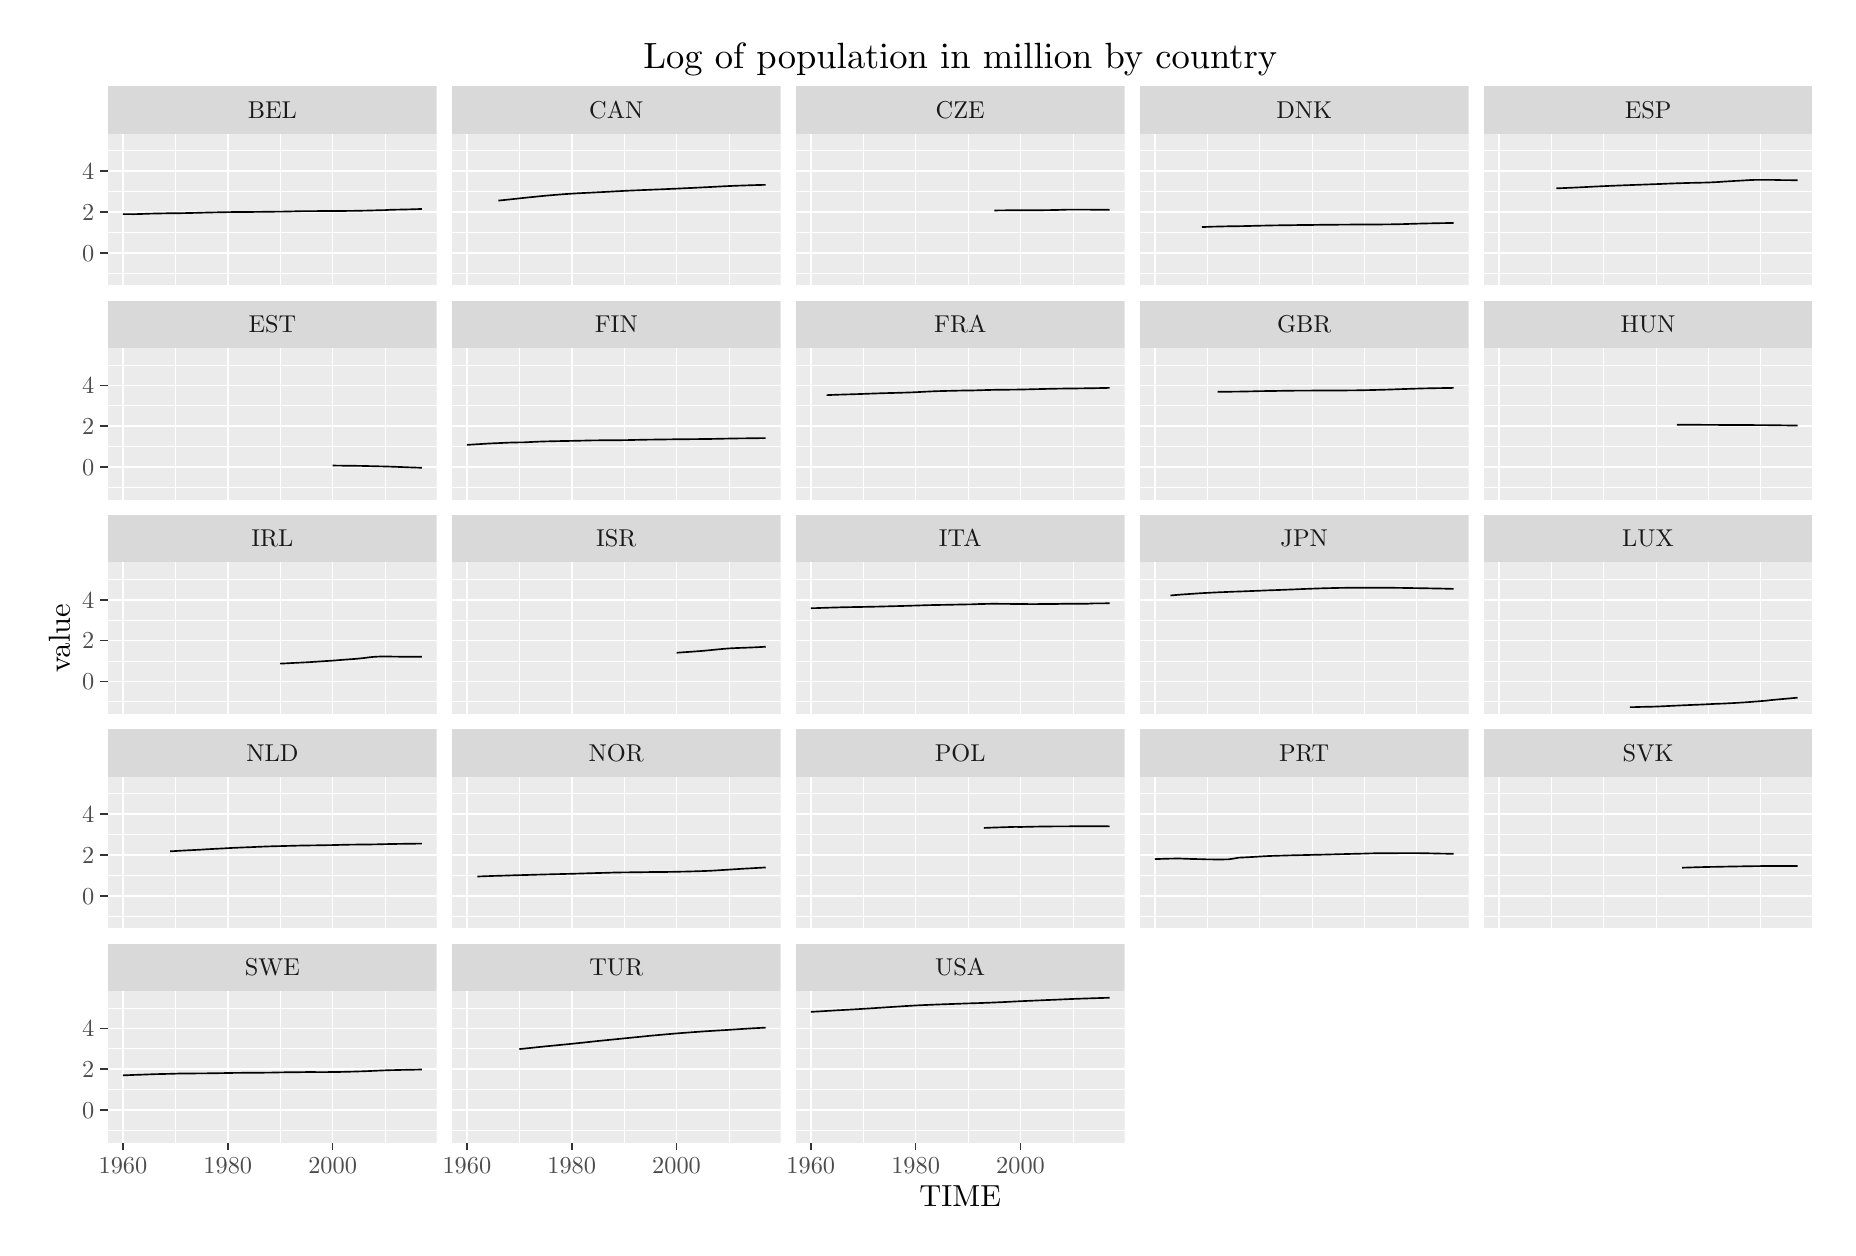
\begin{tikzpicture}[x=1pt,y=1pt]
\definecolor{fillColor}{RGB}{255,255,255}
\path[use as bounding box,fill=fillColor,fill opacity=0.00] (0,0) rectangle (650.43,433.62);
\begin{scope}
\path[clip] (  0.00,  0.00) rectangle (650.43,433.62);
\definecolor{drawColor}{RGB}{255,255,255}
\definecolor{fillColor}{RGB}{255,255,255}

\path[draw=drawColor,line width= 0.6pt,line join=round,line cap=round,fill=fillColor] (  0.00,  0.00) rectangle (650.43,433.62);
\end{scope}
\begin{scope}
\path[clip] ( 29.02,340.48) rectangle (147.81,395.37);
\definecolor{fillColor}{gray}{0.92}

\path[fill=fillColor] ( 29.02,340.48) rectangle (147.81,395.37);
\definecolor{drawColor}{RGB}{255,255,255}

\path[draw=drawColor,line width= 0.3pt,line join=round] ( 29.02,344.93) --
	(147.81,344.93);

\path[draw=drawColor,line width= 0.3pt,line join=round] ( 29.02,359.67) --
	(147.81,359.67);

\path[draw=drawColor,line width= 0.3pt,line join=round] ( 29.02,374.42) --
	(147.81,374.42);

\path[draw=drawColor,line width= 0.3pt,line join=round] ( 29.02,389.17) --
	(147.81,389.17);

\path[draw=drawColor,line width= 0.3pt,line join=round] ( 53.37,340.48) --
	( 53.37,395.37);

\path[draw=drawColor,line width= 0.3pt,line join=round] ( 91.26,340.48) --
	( 91.26,395.37);

\path[draw=drawColor,line width= 0.3pt,line join=round] (129.15,340.48) --
	(129.15,395.37);

\path[draw=drawColor,line width= 0.6pt,line join=round] ( 29.02,352.30) --
	(147.81,352.30);

\path[draw=drawColor,line width= 0.6pt,line join=round] ( 29.02,367.05) --
	(147.81,367.05);

\path[draw=drawColor,line width= 0.6pt,line join=round] ( 29.02,381.79) --
	(147.81,381.79);

\path[draw=drawColor,line width= 0.6pt,line join=round] ( 34.42,340.48) --
	( 34.42,395.37);

\path[draw=drawColor,line width= 0.6pt,line join=round] ( 72.31,340.48) --
	( 72.31,395.37);

\path[draw=drawColor,line width= 0.6pt,line join=round] (110.20,340.48) --
	(110.20,395.37);
\definecolor{drawColor}{RGB}{0,0,0}

\path[draw=drawColor,line width= 0.6pt,line join=round] ( 34.42,366.23) --
	( 36.32,366.24) --
	( 38.21,366.22) --
	( 40.11,366.27) --
	( 42.00,366.33) --
	( 43.90,366.40) --
	( 45.79,366.45) --
	( 47.69,366.48) --
	( 49.58,366.52) --
	( 51.47,366.55) --
	( 53.37,366.58) --
	( 55.26,366.58) --
	( 57.16,366.62) --
	( 59.05,366.66) --
	( 60.95,366.70) --
	( 62.84,366.76) --
	( 64.73,366.81) --
	( 66.63,366.85) --
	( 68.52,366.89) --
	( 70.42,366.92) --
	( 72.31,366.96) --
	( 74.21,366.99) --
	( 76.10,366.99) --
	( 78.00,367.01) --
	( 79.89,367.01) --
	( 81.78,367.04) --
	( 83.68,367.06) --
	( 85.57,367.08) --
	( 87.47,367.09) --
	( 89.36,367.13) --
	( 91.26,367.14) --
	( 93.15,367.17) --
	( 95.05,367.21) --
	( 96.94,367.26) --
	( 98.83,367.31) --
	(100.73,367.33) --
	(102.62,367.33) --
	(104.52,367.34) --
	(106.41,367.35) --
	(108.31,367.35) --
	(110.20,367.35) --
	(112.10,367.35) --
	(113.99,367.38) --
	(115.88,367.41) --
	(117.78,367.43) --
	(119.67,367.46) --
	(121.57,367.50) --
	(123.46,367.54) --
	(125.36,367.60) --
	(127.25,367.65) --
	(129.15,367.69) --
	(131.04,367.80) --
	(132.93,367.85) --
	(134.83,367.89) --
	(136.72,367.93) --
	(138.62,367.98) --
	(140.51,368.04) --
	(142.41,368.11);
\end{scope}
\begin{scope}
\path[clip] (153.31,340.48) rectangle (272.09,395.37);
\definecolor{fillColor}{gray}{0.92}

\path[fill=fillColor] (153.31,340.48) rectangle (272.09,395.37);
\definecolor{drawColor}{RGB}{255,255,255}

\path[draw=drawColor,line width= 0.3pt,line join=round] (153.31,344.93) --
	(272.09,344.93);

\path[draw=drawColor,line width= 0.3pt,line join=round] (153.31,359.67) --
	(272.09,359.67);

\path[draw=drawColor,line width= 0.3pt,line join=round] (153.31,374.42) --
	(272.09,374.42);

\path[draw=drawColor,line width= 0.3pt,line join=round] (153.31,389.17) --
	(272.09,389.17);

\path[draw=drawColor,line width= 0.3pt,line join=round] (177.65,340.48) --
	(177.65,395.37);

\path[draw=drawColor,line width= 0.3pt,line join=round] (215.54,340.48) --
	(215.54,395.37);

\path[draw=drawColor,line width= 0.3pt,line join=round] (253.43,340.48) --
	(253.43,395.37);

\path[draw=drawColor,line width= 0.6pt,line join=round] (153.31,352.30) --
	(272.09,352.30);

\path[draw=drawColor,line width= 0.6pt,line join=round] (153.31,367.05) --
	(272.09,367.05);

\path[draw=drawColor,line width= 0.6pt,line join=round] (153.31,381.79) --
	(272.09,381.79);

\path[draw=drawColor,line width= 0.6pt,line join=round] (158.71,340.48) --
	(158.71,395.37);

\path[draw=drawColor,line width= 0.6pt,line join=round] (196.59,340.48) --
	(196.59,395.37);

\path[draw=drawColor,line width= 0.6pt,line join=round] (234.48,340.48) --
	(234.48,395.37);
\definecolor{drawColor}{RGB}{0,0,0}

\path[draw=drawColor,line width= 0.6pt,line join=round] (170.07,371.13) --
	(171.97,371.32) --
	(173.86,371.52) --
	(175.75,371.72) --
	(177.65,371.92) --
	(179.54,372.13) --
	(181.44,372.33) --
	(183.33,372.52) --
	(185.23,372.71) --
	(187.12,372.90) --
	(189.02,373.06) --
	(190.91,373.22) --
	(192.80,373.37) --
	(194.70,373.51) --
	(196.59,373.64) --
	(198.49,373.75) --
	(200.38,373.85) --
	(202.28,373.94) --
	(204.17,374.04) --
	(206.07,374.13) --
	(207.96,374.23) --
	(209.85,374.33) --
	(211.75,374.44) --
	(213.64,374.54) --
	(215.54,374.64) --
	(217.43,374.73) --
	(219.33,374.81) --
	(221.22,374.89) --
	(223.12,374.97) --
	(225.01,375.05) --
	(226.90,375.13) --
	(228.80,375.20) --
	(230.69,375.28) --
	(232.59,375.37) --
	(234.48,375.45) --
	(236.38,375.54) --
	(238.27,375.63) --
	(240.17,375.71) --
	(242.06,375.81) --
	(243.95,375.91) --
	(245.85,376.00) --
	(247.74,376.10) --
	(249.64,376.20) --
	(251.53,376.30) --
	(253.43,376.39) --
	(255.32,376.47) --
	(257.22,376.54) --
	(259.11,376.60) --
	(261.00,376.67) --
	(262.90,376.73) --
	(264.79,376.78) --
	(266.69,376.83);
\end{scope}
\begin{scope}
\path[clip] (277.59,340.48) rectangle (396.37,395.37);
\definecolor{fillColor}{gray}{0.92}

\path[fill=fillColor] (277.59,340.48) rectangle (396.37,395.37);
\definecolor{drawColor}{RGB}{255,255,255}

\path[draw=drawColor,line width= 0.3pt,line join=round] (277.59,344.93) --
	(396.37,344.93);

\path[draw=drawColor,line width= 0.3pt,line join=round] (277.59,359.67) --
	(396.37,359.67);

\path[draw=drawColor,line width= 0.3pt,line join=round] (277.59,374.42) --
	(396.37,374.42);

\path[draw=drawColor,line width= 0.3pt,line join=round] (277.59,389.17) --
	(396.37,389.17);

\path[draw=drawColor,line width= 0.3pt,line join=round] (301.93,340.48) --
	(301.93,395.37);

\path[draw=drawColor,line width= 0.3pt,line join=round] (339.82,340.48) --
	(339.82,395.37);

\path[draw=drawColor,line width= 0.3pt,line join=round] (377.71,340.48) --
	(377.71,395.37);

\path[draw=drawColor,line width= 0.6pt,line join=round] (277.59,352.30) --
	(396.37,352.30);

\path[draw=drawColor,line width= 0.6pt,line join=round] (277.59,367.05) --
	(396.37,367.05);

\path[draw=drawColor,line width= 0.6pt,line join=round] (277.59,381.79) --
	(396.37,381.79);

\path[draw=drawColor,line width= 0.6pt,line join=round] (282.99,340.48) --
	(282.99,395.37);

\path[draw=drawColor,line width= 0.6pt,line join=round] (320.87,340.48) --
	(320.87,395.37);

\path[draw=drawColor,line width= 0.6pt,line join=round] (358.76,340.48) --
	(358.76,395.37);
\definecolor{drawColor}{RGB}{0,0,0}

\path[draw=drawColor,line width= 0.6pt,line join=round] (349.29,367.56) --
	(351.19,367.59) --
	(353.08,367.61) --
	(354.97,367.62) --
	(356.87,367.63) --
	(358.76,367.65) --
	(360.66,367.64) --
	(362.55,367.63) --
	(364.45,367.64) --
	(366.34,367.66) --
	(368.24,367.68) --
	(370.13,367.71) --
	(372.02,367.74) --
	(373.92,367.81) --
	(375.81,367.87) --
	(377.71,367.88) --
	(379.60,367.88) --
	(381.50,367.87) --
	(383.39,367.86) --
	(385.29,367.83) --
	(387.18,367.82) --
	(389.07,367.81) --
	(390.97,367.79);
\end{scope}
\begin{scope}
\path[clip] (401.87,340.48) rectangle (520.65,395.37);
\definecolor{fillColor}{gray}{0.92}

\path[fill=fillColor] (401.87,340.48) rectangle (520.65,395.37);
\definecolor{drawColor}{RGB}{255,255,255}

\path[draw=drawColor,line width= 0.3pt,line join=round] (401.87,344.93) --
	(520.65,344.93);

\path[draw=drawColor,line width= 0.3pt,line join=round] (401.87,359.67) --
	(520.65,359.67);

\path[draw=drawColor,line width= 0.3pt,line join=round] (401.87,374.42) --
	(520.65,374.42);

\path[draw=drawColor,line width= 0.3pt,line join=round] (401.87,389.17) --
	(520.65,389.17);

\path[draw=drawColor,line width= 0.3pt,line join=round] (426.21,340.48) --
	(426.21,395.37);

\path[draw=drawColor,line width= 0.3pt,line join=round] (464.10,340.48) --
	(464.10,395.37);

\path[draw=drawColor,line width= 0.3pt,line join=round] (501.99,340.48) --
	(501.99,395.37);

\path[draw=drawColor,line width= 0.6pt,line join=round] (401.87,352.30) --
	(520.65,352.30);

\path[draw=drawColor,line width= 0.6pt,line join=round] (401.87,367.05) --
	(520.65,367.05);

\path[draw=drawColor,line width= 0.6pt,line join=round] (401.87,381.79) --
	(520.65,381.79);

\path[draw=drawColor,line width= 0.6pt,line join=round] (407.27,340.48) --
	(407.27,395.37);

\path[draw=drawColor,line width= 0.6pt,line join=round] (445.16,340.48) --
	(445.16,395.37);

\path[draw=drawColor,line width= 0.6pt,line join=round] (483.04,340.48) --
	(483.04,395.37);
\definecolor{drawColor}{RGB}{0,0,0}

\path[draw=drawColor,line width= 0.6pt,line join=round] (424.32,361.58) --
	(426.21,361.63) --
	(428.11,361.71) --
	(430.00,361.75) --
	(431.89,361.79) --
	(433.79,361.84) --
	(435.68,361.87) --
	(437.58,361.88) --
	(439.47,361.92) --
	(441.37,361.96) --
	(443.26,362.01) --
	(445.16,362.06) --
	(447.05,362.10) --
	(448.94,362.14) --
	(450.84,362.18) --
	(452.73,362.20) --
	(454.63,362.22) --
	(456.52,362.24) --
	(458.42,362.28) --
	(460.31,362.30) --
	(462.21,362.32) --
	(464.10,362.33) --
	(465.99,362.36) --
	(467.89,362.39) --
	(469.78,362.40) --
	(471.68,362.42) --
	(473.57,362.43) --
	(475.47,362.46) --
	(477.36,362.46) --
	(479.26,362.47) --
	(481.15,362.47) --
	(483.04,362.47) --
	(484.94,362.48) --
	(486.83,362.49) --
	(488.73,362.51) --
	(490.62,362.53) --
	(492.52,362.55) --
	(494.41,362.58) --
	(496.31,362.62) --
	(498.20,362.67) --
	(500.09,362.74) --
	(501.99,362.79) --
	(503.88,362.84) --
	(505.78,362.88) --
	(507.67,362.92) --
	(509.57,362.96) --
	(511.46,362.99) --
	(513.36,363.02) --
	(515.25,363.04);
\end{scope}
\begin{scope}
\path[clip] (526.15,340.48) rectangle (644.93,395.37);
\definecolor{fillColor}{gray}{0.92}

\path[fill=fillColor] (526.15,340.48) rectangle (644.93,395.37);
\definecolor{drawColor}{RGB}{255,255,255}

\path[draw=drawColor,line width= 0.3pt,line join=round] (526.15,344.93) --
	(644.93,344.93);

\path[draw=drawColor,line width= 0.3pt,line join=round] (526.15,359.67) --
	(644.93,359.67);

\path[draw=drawColor,line width= 0.3pt,line join=round] (526.15,374.42) --
	(644.93,374.42);

\path[draw=drawColor,line width= 0.3pt,line join=round] (526.15,389.17) --
	(644.93,389.17);

\path[draw=drawColor,line width= 0.3pt,line join=round] (550.49,340.48) --
	(550.49,395.37);

\path[draw=drawColor,line width= 0.3pt,line join=round] (588.38,340.48) --
	(588.38,395.37);

\path[draw=drawColor,line width= 0.3pt,line join=round] (626.27,340.48) --
	(626.27,395.37);

\path[draw=drawColor,line width= 0.6pt,line join=round] (526.15,352.30) --
	(644.93,352.30);

\path[draw=drawColor,line width= 0.6pt,line join=round] (526.15,367.05) --
	(644.93,367.05);

\path[draw=drawColor,line width= 0.6pt,line join=round] (526.15,381.79) --
	(644.93,381.79);

\path[draw=drawColor,line width= 0.6pt,line join=round] (531.55,340.48) --
	(531.55,395.37);

\path[draw=drawColor,line width= 0.6pt,line join=round] (569.44,340.48) --
	(569.44,395.37);

\path[draw=drawColor,line width= 0.6pt,line join=round] (607.33,340.48) --
	(607.33,395.37);
\definecolor{drawColor}{RGB}{0,0,0}

\path[draw=drawColor,line width= 0.6pt,line join=round] (552.39,375.56) --
	(554.28,375.63) --
	(556.18,375.71) --
	(558.07,375.79) --
	(559.96,375.88) --
	(561.86,375.97) --
	(563.75,376.07) --
	(565.65,376.17) --
	(567.54,376.26) --
	(569.44,376.35) --
	(571.33,376.43) --
	(573.23,376.51) --
	(575.12,376.59) --
	(577.01,376.66) --
	(578.91,376.73) --
	(580.80,376.80) --
	(582.70,376.87) --
	(584.59,376.94) --
	(586.49,377.01) --
	(588.38,377.08) --
	(590.28,377.15) --
	(592.17,377.24) --
	(594.06,377.31) --
	(595.96,377.38) --
	(597.85,377.44) --
	(599.75,377.50) --
	(601.64,377.54) --
	(603.54,377.58) --
	(605.43,377.62) --
	(607.33,377.67) --
	(609.22,377.76) --
	(611.11,377.86) --
	(613.01,378.00) --
	(614.90,378.11) --
	(616.80,378.23) --
	(618.69,378.33) --
	(620.59,378.44) --
	(622.48,378.56) --
	(624.38,378.62) --
	(626.27,378.63) --
	(628.16,378.63) --
	(630.06,378.62) --
	(631.95,378.59) --
	(633.85,378.53) --
	(635.74,378.53) --
	(637.64,378.50) --
	(639.53,378.49);
\end{scope}
\begin{scope}
\path[clip] ( 29.02,263.03) rectangle (147.81,317.92);
\definecolor{fillColor}{gray}{0.92}

\path[fill=fillColor] ( 29.02,263.03) rectangle (147.81,317.92);
\definecolor{drawColor}{RGB}{255,255,255}

\path[draw=drawColor,line width= 0.3pt,line join=round] ( 29.02,267.48) --
	(147.81,267.48);

\path[draw=drawColor,line width= 0.3pt,line join=round] ( 29.02,282.23) --
	(147.81,282.23);

\path[draw=drawColor,line width= 0.3pt,line join=round] ( 29.02,296.97) --
	(147.81,296.97);

\path[draw=drawColor,line width= 0.3pt,line join=round] ( 29.02,311.72) --
	(147.81,311.72);

\path[draw=drawColor,line width= 0.3pt,line join=round] ( 53.37,263.03) --
	( 53.37,317.92);

\path[draw=drawColor,line width= 0.3pt,line join=round] ( 91.26,263.03) --
	( 91.26,317.92);

\path[draw=drawColor,line width= 0.3pt,line join=round] (129.15,263.03) --
	(129.15,317.92);

\path[draw=drawColor,line width= 0.6pt,line join=round] ( 29.02,274.85) --
	(147.81,274.85);

\path[draw=drawColor,line width= 0.6pt,line join=round] ( 29.02,289.60) --
	(147.81,289.60);

\path[draw=drawColor,line width= 0.6pt,line join=round] ( 29.02,304.34) --
	(147.81,304.34);

\path[draw=drawColor,line width= 0.6pt,line join=round] ( 34.42,263.03) --
	( 34.42,317.92);

\path[draw=drawColor,line width= 0.6pt,line join=round] ( 72.31,263.03) --
	( 72.31,317.92);

\path[draw=drawColor,line width= 0.6pt,line join=round] (110.20,263.03) --
	(110.20,317.92);
\definecolor{drawColor}{RGB}{0,0,0}

\path[draw=drawColor,line width= 0.6pt,line join=round] (110.20,275.39) --
	(112.10,275.37) --
	(113.99,275.34) --
	(115.88,275.32) --
	(117.78,275.30) --
	(119.67,275.28) --
	(121.57,275.24) --
	(123.46,275.19) --
	(125.36,275.14) --
	(127.25,275.10) --
	(129.15,275.06) --
	(131.04,275.00) --
	(132.93,274.93) --
	(134.83,274.86) --
	(136.72,274.78) --
	(138.62,274.71) --
	(140.51,274.65) --
	(142.41,274.58);
\end{scope}
\begin{scope}
\path[clip] (153.31,263.03) rectangle (272.09,317.92);
\definecolor{fillColor}{gray}{0.92}

\path[fill=fillColor] (153.31,263.03) rectangle (272.09,317.92);
\definecolor{drawColor}{RGB}{255,255,255}

\path[draw=drawColor,line width= 0.3pt,line join=round] (153.31,267.48) --
	(272.09,267.48);

\path[draw=drawColor,line width= 0.3pt,line join=round] (153.31,282.23) --
	(272.09,282.23);

\path[draw=drawColor,line width= 0.3pt,line join=round] (153.31,296.97) --
	(272.09,296.97);

\path[draw=drawColor,line width= 0.3pt,line join=round] (153.31,311.72) --
	(272.09,311.72);

\path[draw=drawColor,line width= 0.3pt,line join=round] (177.65,263.03) --
	(177.65,317.92);

\path[draw=drawColor,line width= 0.3pt,line join=round] (215.54,263.03) --
	(215.54,317.92);

\path[draw=drawColor,line width= 0.3pt,line join=round] (253.43,263.03) --
	(253.43,317.92);

\path[draw=drawColor,line width= 0.6pt,line join=round] (153.31,274.85) --
	(272.09,274.85);

\path[draw=drawColor,line width= 0.6pt,line join=round] (153.31,289.60) --
	(272.09,289.60);

\path[draw=drawColor,line width= 0.6pt,line join=round] (153.31,304.34) --
	(272.09,304.34);

\path[draw=drawColor,line width= 0.6pt,line join=round] (158.71,263.03) --
	(158.71,317.92);

\path[draw=drawColor,line width= 0.6pt,line join=round] (196.59,263.03) --
	(196.59,317.92);

\path[draw=drawColor,line width= 0.6pt,line join=round] (234.48,263.03) --
	(234.48,317.92);
\definecolor{drawColor}{RGB}{0,0,0}

\path[draw=drawColor,line width= 0.6pt,line join=round] (158.71,282.86) --
	(160.60,282.97) --
	(162.49,283.09) --
	(164.39,283.21) --
	(166.28,283.33) --
	(168.18,283.42) --
	(170.07,283.50) --
	(171.97,283.58) --
	(173.86,283.67) --
	(175.75,283.74) --
	(177.65,283.75) --
	(179.54,283.78) --
	(181.44,283.88) --
	(183.33,283.97) --
	(185.23,284.05) --
	(187.12,284.11) --
	(189.02,284.16) --
	(190.91,284.20) --
	(192.80,284.24) --
	(194.70,284.27) --
	(196.59,284.31) --
	(198.49,284.35) --
	(200.38,284.39) --
	(202.28,284.44) --
	(204.17,284.48) --
	(206.07,284.50) --
	(207.96,284.52) --
	(209.85,284.53) --
	(211.75,284.54) --
	(213.64,284.54) --
	(215.54,284.57) --
	(217.43,284.60) --
	(219.33,284.65) --
	(221.22,284.69) --
	(223.12,284.73) --
	(225.01,284.76) --
	(226.90,284.78) --
	(228.80,284.80) --
	(230.69,284.83) --
	(232.59,284.86) --
	(234.48,284.88) --
	(236.38,284.90) --
	(238.27,284.91) --
	(240.17,284.93) --
	(242.06,284.95) --
	(243.95,284.97) --
	(245.85,284.99) --
	(247.74,285.02) --
	(249.64,285.06) --
	(251.53,285.10) --
	(253.43,285.14) --
	(255.32,285.17) --
	(257.22,285.20) --
	(259.11,285.22) --
	(261.00,285.24) --
	(262.90,285.26) --
	(264.79,285.29) --
	(266.69,285.29);
\end{scope}
\begin{scope}
\path[clip] (277.59,263.03) rectangle (396.37,317.92);
\definecolor{fillColor}{gray}{0.92}

\path[fill=fillColor] (277.59,263.03) rectangle (396.37,317.92);
\definecolor{drawColor}{RGB}{255,255,255}

\path[draw=drawColor,line width= 0.3pt,line join=round] (277.59,267.48) --
	(396.37,267.48);

\path[draw=drawColor,line width= 0.3pt,line join=round] (277.59,282.23) --
	(396.37,282.23);

\path[draw=drawColor,line width= 0.3pt,line join=round] (277.59,296.97) --
	(396.37,296.97);

\path[draw=drawColor,line width= 0.3pt,line join=round] (277.59,311.72) --
	(396.37,311.72);

\path[draw=drawColor,line width= 0.3pt,line join=round] (301.93,263.03) --
	(301.93,317.92);

\path[draw=drawColor,line width= 0.3pt,line join=round] (339.82,263.03) --
	(339.82,317.92);

\path[draw=drawColor,line width= 0.3pt,line join=round] (377.71,263.03) --
	(377.71,317.92);

\path[draw=drawColor,line width= 0.6pt,line join=round] (277.59,274.85) --
	(396.37,274.85);

\path[draw=drawColor,line width= 0.6pt,line join=round] (277.59,289.60) --
	(396.37,289.60);

\path[draw=drawColor,line width= 0.6pt,line join=round] (277.59,304.34) --
	(396.37,304.34);

\path[draw=drawColor,line width= 0.6pt,line join=round] (282.99,263.03) --
	(282.99,317.92);

\path[draw=drawColor,line width= 0.6pt,line join=round] (320.87,263.03) --
	(320.87,317.92);

\path[draw=drawColor,line width= 0.6pt,line join=round] (358.76,263.03) --
	(358.76,317.92);
\definecolor{drawColor}{RGB}{0,0,0}

\path[draw=drawColor,line width= 0.6pt,line join=round] (288.67,300.83) --
	(290.56,300.91) --
	(292.46,300.98) --
	(294.35,301.04) --
	(296.25,301.10) --
	(298.14,301.15) --
	(300.04,301.21) --
	(301.93,301.28) --
	(303.82,301.35) --
	(305.72,301.42) --
	(307.61,301.48) --
	(309.51,301.54) --
	(311.40,301.59) --
	(313.30,301.64) --
	(315.19,301.70) --
	(317.09,301.75) --
	(318.98,301.81) --
	(320.87,301.89) --
	(322.77,301.99) --
	(324.66,302.09) --
	(326.56,302.18) --
	(328.45,302.26) --
	(330.35,302.32) --
	(332.24,302.36) --
	(334.14,302.40) --
	(336.03,302.45) --
	(337.92,302.49) --
	(339.82,302.51) --
	(341.71,302.53) --
	(343.61,302.59) --
	(345.50,302.65) --
	(347.40,302.70) --
	(349.29,302.75) --
	(351.19,302.77) --
	(353.08,302.79) --
	(354.97,302.81) --
	(356.87,302.83) --
	(358.76,302.86) --
	(360.66,302.90) --
	(362.55,302.95) --
	(364.45,303.00) --
	(366.34,303.04) --
	(368.24,303.09) --
	(370.13,303.14) --
	(372.02,303.17) --
	(373.92,303.20) --
	(375.81,303.22) --
	(377.71,303.24) --
	(379.60,303.26) --
	(381.50,303.29) --
	(383.39,303.31) --
	(385.29,303.34) --
	(387.18,303.38) --
	(389.07,303.42) --
	(390.97,303.46);
\end{scope}
\begin{scope}
\path[clip] (401.87,263.03) rectangle (520.65,317.92);
\definecolor{fillColor}{gray}{0.92}

\path[fill=fillColor] (401.87,263.03) rectangle (520.65,317.92);
\definecolor{drawColor}{RGB}{255,255,255}

\path[draw=drawColor,line width= 0.3pt,line join=round] (401.87,267.48) --
	(520.65,267.48);

\path[draw=drawColor,line width= 0.3pt,line join=round] (401.87,282.23) --
	(520.65,282.23);

\path[draw=drawColor,line width= 0.3pt,line join=round] (401.87,296.97) --
	(520.65,296.97);

\path[draw=drawColor,line width= 0.3pt,line join=round] (401.87,311.72) --
	(520.65,311.72);

\path[draw=drawColor,line width= 0.3pt,line join=round] (426.21,263.03) --
	(426.21,317.92);

\path[draw=drawColor,line width= 0.3pt,line join=round] (464.10,263.03) --
	(464.10,317.92);

\path[draw=drawColor,line width= 0.3pt,line join=round] (501.99,263.03) --
	(501.99,317.92);

\path[draw=drawColor,line width= 0.6pt,line join=round] (401.87,274.85) --
	(520.65,274.85);

\path[draw=drawColor,line width= 0.6pt,line join=round] (401.87,289.60) --
	(520.65,289.60);

\path[draw=drawColor,line width= 0.6pt,line join=round] (401.87,304.34) --
	(520.65,304.34);

\path[draw=drawColor,line width= 0.6pt,line join=round] (407.27,263.03) --
	(407.27,317.92);

\path[draw=drawColor,line width= 0.6pt,line join=round] (445.16,263.03) --
	(445.16,317.92);

\path[draw=drawColor,line width= 0.6pt,line join=round] (483.04,263.03) --
	(483.04,317.92);
\definecolor{drawColor}{RGB}{0,0,0}

\path[draw=drawColor,line width= 0.6pt,line join=round] (430.00,302.03) --
	(431.89,302.05) --
	(433.79,302.07) --
	(435.68,302.09) --
	(437.58,302.11) --
	(439.47,302.15) --
	(441.37,302.18) --
	(443.26,302.22) --
	(445.16,302.27) --
	(447.05,302.30) --
	(448.94,302.33) --
	(450.84,302.35) --
	(452.73,302.38) --
	(454.63,302.41) --
	(456.52,302.43) --
	(458.42,302.46) --
	(460.31,302.47) --
	(462.21,302.47) --
	(464.10,302.48) --
	(465.99,302.48) --
	(467.89,302.49) --
	(469.78,302.49) --
	(471.68,302.51) --
	(473.57,302.53) --
	(475.47,302.53) --
	(477.36,302.54) --
	(479.26,302.56) --
	(481.15,302.58) --
	(483.04,302.62) --
	(484.94,302.66) --
	(486.83,302.71) --
	(488.73,302.76) --
	(490.62,302.81) --
	(492.52,302.87) --
	(494.41,302.94) --
	(496.31,303.01) --
	(498.20,303.07) --
	(500.09,303.13) --
	(501.99,303.19) --
	(503.88,303.25) --
	(505.78,303.29) --
	(507.67,303.33) --
	(509.57,303.36) --
	(511.46,303.39) --
	(513.36,303.42) --
	(515.25,303.45);
\end{scope}
\begin{scope}
\path[clip] (526.15,263.03) rectangle (644.93,317.92);
\definecolor{fillColor}{gray}{0.92}

\path[fill=fillColor] (526.15,263.03) rectangle (644.93,317.92);
\definecolor{drawColor}{RGB}{255,255,255}

\path[draw=drawColor,line width= 0.3pt,line join=round] (526.15,267.48) --
	(644.93,267.48);

\path[draw=drawColor,line width= 0.3pt,line join=round] (526.15,282.23) --
	(644.93,282.23);

\path[draw=drawColor,line width= 0.3pt,line join=round] (526.15,296.97) --
	(644.93,296.97);

\path[draw=drawColor,line width= 0.3pt,line join=round] (526.15,311.72) --
	(644.93,311.72);

\path[draw=drawColor,line width= 0.3pt,line join=round] (550.49,263.03) --
	(550.49,317.92);

\path[draw=drawColor,line width= 0.3pt,line join=round] (588.38,263.03) --
	(588.38,317.92);

\path[draw=drawColor,line width= 0.3pt,line join=round] (626.27,263.03) --
	(626.27,317.92);

\path[draw=drawColor,line width= 0.6pt,line join=round] (526.15,274.85) --
	(644.93,274.85);

\path[draw=drawColor,line width= 0.6pt,line join=round] (526.15,289.60) --
	(644.93,289.60);

\path[draw=drawColor,line width= 0.6pt,line join=round] (526.15,304.34) --
	(644.93,304.34);

\path[draw=drawColor,line width= 0.6pt,line join=round] (531.55,263.03) --
	(531.55,317.92);

\path[draw=drawColor,line width= 0.6pt,line join=round] (569.44,263.03) --
	(569.44,317.92);

\path[draw=drawColor,line width= 0.6pt,line join=round] (607.33,263.03) --
	(607.33,317.92);
\definecolor{drawColor}{RGB}{0,0,0}

\path[draw=drawColor,line width= 0.6pt,line join=round] (595.96,290.12) --
	(597.85,290.13) --
	(599.75,290.13) --
	(601.64,290.13) --
	(603.54,290.11) --
	(605.43,290.10) --
	(607.33,290.09) --
	(609.22,290.08) --
	(611.11,290.07) --
	(613.01,290.06) --
	(614.90,290.04) --
	(616.80,290.04) --
	(618.69,290.03) --
	(620.59,290.03) --
	(622.48,290.02) --
	(624.38,290.01) --
	(626.27,290.00) --
	(628.16,289.99) --
	(630.06,289.96) --
	(631.95,289.95) --
	(633.85,289.92) --
	(635.74,289.89) --
	(637.64,289.87) --
	(639.53,289.85);
\end{scope}
\begin{scope}
\path[clip] ( 29.02,185.58) rectangle (147.81,240.47);
\definecolor{fillColor}{gray}{0.92}

\path[fill=fillColor] ( 29.02,185.58) rectangle (147.81,240.47);
\definecolor{drawColor}{RGB}{255,255,255}

\path[draw=drawColor,line width= 0.3pt,line join=round] ( 29.02,190.03) --
	(147.81,190.03);

\path[draw=drawColor,line width= 0.3pt,line join=round] ( 29.02,204.78) --
	(147.81,204.78);

\path[draw=drawColor,line width= 0.3pt,line join=round] ( 29.02,219.52) --
	(147.81,219.52);

\path[draw=drawColor,line width= 0.3pt,line join=round] ( 29.02,234.27) --
	(147.81,234.27);

\path[draw=drawColor,line width= 0.3pt,line join=round] ( 53.37,185.58) --
	( 53.37,240.47);

\path[draw=drawColor,line width= 0.3pt,line join=round] ( 91.26,185.58) --
	( 91.26,240.47);

\path[draw=drawColor,line width= 0.3pt,line join=round] (129.15,185.58) --
	(129.15,240.47);

\path[draw=drawColor,line width= 0.6pt,line join=round] ( 29.02,197.41) --
	(147.81,197.41);

\path[draw=drawColor,line width= 0.6pt,line join=round] ( 29.02,212.15) --
	(147.81,212.15);

\path[draw=drawColor,line width= 0.6pt,line join=round] ( 29.02,226.90) --
	(147.81,226.90);

\path[draw=drawColor,line width= 0.6pt,line join=round] ( 34.42,185.58) --
	( 34.42,240.47);

\path[draw=drawColor,line width= 0.6pt,line join=round] ( 72.31,185.58) --
	( 72.31,240.47);

\path[draw=drawColor,line width= 0.6pt,line join=round] (110.20,185.58) --
	(110.20,240.47);
\definecolor{drawColor}{RGB}{0,0,0}

\path[draw=drawColor,line width= 0.6pt,line join=round] ( 91.26,203.82) --
	( 93.15,203.90) --
	( 95.05,204.01) --
	( 96.94,204.11) --
	( 98.83,204.20) --
	(100.73,204.29) --
	(102.62,204.40) --
	(104.52,204.53) --
	(106.41,204.66) --
	(108.31,204.78) --
	(110.20,204.90) --
	(112.10,205.05) --
	(113.99,205.21) --
	(115.88,205.35) --
	(117.78,205.48) --
	(119.67,205.65) --
	(121.57,205.85) --
	(123.46,206.10) --
	(125.36,206.30) --
	(127.25,206.37) --
	(129.15,206.37) --
	(131.04,206.37) --
	(132.93,206.34) --
	(134.83,206.32) --
	(136.72,206.31) --
	(138.62,206.30) --
	(140.51,206.30) --
	(142.41,206.29);
\end{scope}
\begin{scope}
\path[clip] (153.31,185.58) rectangle (272.09,240.47);
\definecolor{fillColor}{gray}{0.92}

\path[fill=fillColor] (153.31,185.58) rectangle (272.09,240.47);
\definecolor{drawColor}{RGB}{255,255,255}

\path[draw=drawColor,line width= 0.3pt,line join=round] (153.31,190.03) --
	(272.09,190.03);

\path[draw=drawColor,line width= 0.3pt,line join=round] (153.31,204.78) --
	(272.09,204.78);

\path[draw=drawColor,line width= 0.3pt,line join=round] (153.31,219.52) --
	(272.09,219.52);

\path[draw=drawColor,line width= 0.3pt,line join=round] (153.31,234.27) --
	(272.09,234.27);

\path[draw=drawColor,line width= 0.3pt,line join=round] (177.65,185.58) --
	(177.65,240.47);

\path[draw=drawColor,line width= 0.3pt,line join=round] (215.54,185.58) --
	(215.54,240.47);

\path[draw=drawColor,line width= 0.3pt,line join=round] (253.43,185.58) --
	(253.43,240.47);

\path[draw=drawColor,line width= 0.6pt,line join=round] (153.31,197.41) --
	(272.09,197.41);

\path[draw=drawColor,line width= 0.6pt,line join=round] (153.31,212.15) --
	(272.09,212.15);

\path[draw=drawColor,line width= 0.6pt,line join=round] (153.31,226.90) --
	(272.09,226.90);

\path[draw=drawColor,line width= 0.6pt,line join=round] (158.71,185.58) --
	(158.71,240.47);

\path[draw=drawColor,line width= 0.6pt,line join=round] (196.59,185.58) --
	(196.59,240.47);

\path[draw=drawColor,line width= 0.6pt,line join=round] (234.48,185.58) --
	(234.48,240.47);
\definecolor{drawColor}{RGB}{0,0,0}

\path[draw=drawColor,line width= 0.6pt,line join=round] (234.48,207.75) --
	(236.38,207.88) --
	(238.27,208.01) --
	(240.17,208.14) --
	(242.06,208.28) --
	(243.95,208.43) --
	(245.85,208.61) --
	(247.74,208.80) --
	(249.64,208.98) --
	(251.53,209.16) --
	(253.43,209.31) --
	(255.32,209.41) --
	(257.22,209.49) --
	(259.11,209.56) --
	(261.00,209.63) --
	(262.90,209.71) --
	(264.79,209.81) --
	(266.69,209.93);
\end{scope}
\begin{scope}
\path[clip] (277.59,185.58) rectangle (396.37,240.47);
\definecolor{fillColor}{gray}{0.92}

\path[fill=fillColor] (277.59,185.58) rectangle (396.37,240.47);
\definecolor{drawColor}{RGB}{255,255,255}

\path[draw=drawColor,line width= 0.3pt,line join=round] (277.59,190.03) --
	(396.37,190.03);

\path[draw=drawColor,line width= 0.3pt,line join=round] (277.59,204.78) --
	(396.37,204.78);

\path[draw=drawColor,line width= 0.3pt,line join=round] (277.59,219.52) --
	(396.37,219.52);

\path[draw=drawColor,line width= 0.3pt,line join=round] (277.59,234.27) --
	(396.37,234.27);

\path[draw=drawColor,line width= 0.3pt,line join=round] (301.93,185.58) --
	(301.93,240.47);

\path[draw=drawColor,line width= 0.3pt,line join=round] (339.82,185.58) --
	(339.82,240.47);

\path[draw=drawColor,line width= 0.3pt,line join=round] (377.71,185.58) --
	(377.71,240.47);

\path[draw=drawColor,line width= 0.6pt,line join=round] (277.59,197.41) --
	(396.37,197.41);

\path[draw=drawColor,line width= 0.6pt,line join=round] (277.59,212.15) --
	(396.37,212.15);

\path[draw=drawColor,line width= 0.6pt,line join=round] (277.59,226.90) --
	(396.37,226.90);

\path[draw=drawColor,line width= 0.6pt,line join=round] (282.99,185.58) --
	(282.99,240.47);

\path[draw=drawColor,line width= 0.6pt,line join=round] (320.87,185.58) --
	(320.87,240.47);

\path[draw=drawColor,line width= 0.6pt,line join=round] (358.76,185.58) --
	(358.76,240.47);
\definecolor{drawColor}{RGB}{0,0,0}

\path[draw=drawColor,line width= 0.6pt,line join=round] (282.99,223.84) --
	(284.88,223.88) --
	(286.77,223.95) --
	(288.67,224.01) --
	(290.56,224.07) --
	(292.46,224.12) --
	(294.35,224.18) --
	(296.25,224.21) --
	(298.14,224.25) --
	(300.04,224.28) --
	(301.93,224.31) --
	(303.82,224.35) --
	(305.72,224.39) --
	(307.61,224.43) --
	(309.51,224.48) --
	(311.40,224.53) --
	(313.30,224.58) --
	(315.19,224.63) --
	(317.09,224.68) --
	(318.98,224.74) --
	(320.87,224.80) --
	(322.77,224.86) --
	(324.66,224.92) --
	(326.56,224.97) --
	(328.45,225.00) --
	(330.35,225.04) --
	(332.24,225.07) --
	(334.14,225.11) --
	(336.03,225.15) --
	(337.92,225.18) --
	(339.82,225.22) --
	(341.71,225.25) --
	(343.61,225.34) --
	(345.50,225.38) --
	(347.40,225.42) --
	(349.29,225.43) --
	(351.19,225.42) --
	(353.08,225.41) --
	(354.97,225.39) --
	(356.87,225.37) --
	(358.76,225.36) --
	(360.66,225.34) --
	(362.55,225.32) --
	(364.45,225.32) --
	(366.34,225.36) --
	(368.24,225.39) --
	(370.13,225.39) --
	(372.02,225.38) --
	(373.92,225.43) --
	(375.81,225.45) --
	(377.71,225.46) --
	(379.60,225.46) --
	(381.50,225.46) --
	(383.39,225.48) --
	(385.29,225.59) --
	(387.18,225.59) --
	(389.07,225.60) --
	(390.97,225.62);
\end{scope}
\begin{scope}
\path[clip] (401.87,185.58) rectangle (520.65,240.47);
\definecolor{fillColor}{gray}{0.92}

\path[fill=fillColor] (401.87,185.58) rectangle (520.65,240.47);
\definecolor{drawColor}{RGB}{255,255,255}

\path[draw=drawColor,line width= 0.3pt,line join=round] (401.87,190.03) --
	(520.65,190.03);

\path[draw=drawColor,line width= 0.3pt,line join=round] (401.87,204.78) --
	(520.65,204.78);

\path[draw=drawColor,line width= 0.3pt,line join=round] (401.87,219.52) --
	(520.65,219.52);

\path[draw=drawColor,line width= 0.3pt,line join=round] (401.87,234.27) --
	(520.65,234.27);

\path[draw=drawColor,line width= 0.3pt,line join=round] (426.21,185.58) --
	(426.21,240.47);

\path[draw=drawColor,line width= 0.3pt,line join=round] (464.10,185.58) --
	(464.10,240.47);

\path[draw=drawColor,line width= 0.3pt,line join=round] (501.99,185.58) --
	(501.99,240.47);

\path[draw=drawColor,line width= 0.6pt,line join=round] (401.87,197.41) --
	(520.65,197.41);

\path[draw=drawColor,line width= 0.6pt,line join=round] (401.87,212.15) --
	(520.65,212.15);

\path[draw=drawColor,line width= 0.6pt,line join=round] (401.87,226.90) --
	(520.65,226.90);

\path[draw=drawColor,line width= 0.6pt,line join=round] (407.27,185.58) --
	(407.27,240.47);

\path[draw=drawColor,line width= 0.6pt,line join=round] (445.16,185.58) --
	(445.16,240.47);

\path[draw=drawColor,line width= 0.6pt,line join=round] (483.04,185.58) --
	(483.04,240.47);
\definecolor{drawColor}{RGB}{0,0,0}

\path[draw=drawColor,line width= 0.6pt,line join=round] (412.95,228.44) --
	(414.84,228.61) --
	(416.74,228.77) --
	(418.63,228.90) --
	(420.53,229.03) --
	(422.42,229.16) --
	(424.32,229.28) --
	(426.21,229.38) --
	(428.11,229.48) --
	(430.00,229.57) --
	(431.89,229.65) --
	(433.79,229.73) --
	(435.68,229.81) --
	(437.58,229.87) --
	(439.47,229.94) --
	(441.37,230.02) --
	(443.26,230.09) --
	(445.16,230.16) --
	(447.05,230.25) --
	(448.94,230.32) --
	(450.84,230.38) --
	(452.73,230.45) --
	(454.63,230.53) --
	(456.52,230.60) --
	(458.42,230.67) --
	(460.31,230.76) --
	(462.21,230.83) --
	(464.10,230.90) --
	(465.99,230.97) --
	(467.89,231.03) --
	(469.78,231.08) --
	(471.68,231.13) --
	(473.57,231.17) --
	(475.47,231.20) --
	(477.36,231.22) --
	(479.26,231.24) --
	(481.15,231.25) --
	(483.04,231.25) --
	(484.94,231.25) --
	(486.83,231.25) --
	(488.73,231.24) --
	(490.62,231.23) --
	(492.52,231.22) --
	(494.41,231.20) --
	(496.31,231.18) --
	(498.20,231.15) --
	(500.09,231.12) --
	(501.99,231.09) --
	(503.88,231.06) --
	(505.78,231.03) --
	(507.67,230.99) --
	(509.57,230.96) --
	(511.46,230.92) --
	(513.36,230.87) --
	(515.25,230.82);
\end{scope}
\begin{scope}
\path[clip] (526.15,185.58) rectangle (644.93,240.47);
\definecolor{fillColor}{gray}{0.92}

\path[fill=fillColor] (526.15,185.58) rectangle (644.93,240.47);
\definecolor{drawColor}{RGB}{255,255,255}

\path[draw=drawColor,line width= 0.3pt,line join=round] (526.15,190.03) --
	(644.93,190.03);

\path[draw=drawColor,line width= 0.3pt,line join=round] (526.15,204.78) --
	(644.93,204.78);

\path[draw=drawColor,line width= 0.3pt,line join=round] (526.15,219.52) --
	(644.93,219.52);

\path[draw=drawColor,line width= 0.3pt,line join=round] (526.15,234.27) --
	(644.93,234.27);

\path[draw=drawColor,line width= 0.3pt,line join=round] (550.49,185.58) --
	(550.49,240.47);

\path[draw=drawColor,line width= 0.3pt,line join=round] (588.38,185.58) --
	(588.38,240.47);

\path[draw=drawColor,line width= 0.3pt,line join=round] (626.27,185.58) --
	(626.27,240.47);

\path[draw=drawColor,line width= 0.6pt,line join=round] (526.15,197.41) --
	(644.93,197.41);

\path[draw=drawColor,line width= 0.6pt,line join=round] (526.15,212.15) --
	(644.93,212.15);

\path[draw=drawColor,line width= 0.6pt,line join=round] (526.15,226.90) --
	(644.93,226.90);

\path[draw=drawColor,line width= 0.6pt,line join=round] (531.55,185.58) --
	(531.55,240.47);

\path[draw=drawColor,line width= 0.6pt,line join=round] (569.44,185.58) --
	(569.44,240.47);

\path[draw=drawColor,line width= 0.6pt,line join=round] (607.33,185.58) --
	(607.33,240.47);
\definecolor{drawColor}{RGB}{0,0,0}

\path[draw=drawColor,line width= 0.6pt,line join=round] (578.91,188.08) --
	(580.80,188.11) --
	(582.70,188.17) --
	(584.59,188.21) --
	(586.49,188.24) --
	(588.38,188.30) --
	(590.28,188.38) --
	(592.17,188.47) --
	(594.06,188.56) --
	(595.96,188.65) --
	(597.85,188.74) --
	(599.75,188.82) --
	(601.64,188.90) --
	(603.54,188.98) --
	(605.43,189.05) --
	(607.33,189.15) --
	(609.22,189.25) --
	(611.11,189.33) --
	(613.01,189.39) --
	(614.90,189.50) --
	(616.80,189.59) --
	(618.69,189.72) --
	(620.59,189.83) --
	(622.48,189.96) --
	(624.38,190.12) --
	(626.27,190.27) --
	(628.16,190.42) --
	(630.06,190.65) --
	(631.95,190.83) --
	(633.85,191.00) --
	(635.74,191.17) --
	(637.64,191.34) --
	(639.53,191.51);
\end{scope}
\begin{scope}
\path[clip] ( 29.02,108.14) rectangle (147.81,163.02);
\definecolor{fillColor}{gray}{0.92}

\path[fill=fillColor] ( 29.02,108.14) rectangle (147.81,163.02);
\definecolor{drawColor}{RGB}{255,255,255}

\path[draw=drawColor,line width= 0.3pt,line join=round] ( 29.02,112.58) --
	(147.81,112.58);

\path[draw=drawColor,line width= 0.3pt,line join=round] ( 29.02,127.33) --
	(147.81,127.33);

\path[draw=drawColor,line width= 0.3pt,line join=round] ( 29.02,142.07) --
	(147.81,142.07);

\path[draw=drawColor,line width= 0.3pt,line join=round] ( 29.02,156.82) --
	(147.81,156.82);

\path[draw=drawColor,line width= 0.3pt,line join=round] ( 53.37,108.14) --
	( 53.37,163.02);

\path[draw=drawColor,line width= 0.3pt,line join=round] ( 91.26,108.14) --
	( 91.26,163.02);

\path[draw=drawColor,line width= 0.3pt,line join=round] (129.15,108.14) --
	(129.15,163.02);

\path[draw=drawColor,line width= 0.6pt,line join=round] ( 29.02,119.96) --
	(147.81,119.96);

\path[draw=drawColor,line width= 0.6pt,line join=round] ( 29.02,134.70) --
	(147.81,134.70);

\path[draw=drawColor,line width= 0.6pt,line join=round] ( 29.02,149.45) --
	(147.81,149.45);

\path[draw=drawColor,line width= 0.6pt,line join=round] ( 34.42,108.14) --
	( 34.42,163.02);

\path[draw=drawColor,line width= 0.6pt,line join=round] ( 72.31,108.14) --
	( 72.31,163.02);

\path[draw=drawColor,line width= 0.6pt,line join=round] (110.20,108.14) --
	(110.20,163.02);
\definecolor{drawColor}{RGB}{0,0,0}

\path[draw=drawColor,line width= 0.6pt,line join=round] ( 51.47,136.00) --
	( 53.37,136.10) --
	( 55.26,136.21) --
	( 57.16,136.32) --
	( 59.05,136.41) --
	( 60.95,136.51) --
	( 62.84,136.61) --
	( 64.73,136.74) --
	( 66.63,136.83) --
	( 68.52,136.93) --
	( 70.42,137.03) --
	( 72.31,137.13) --
	( 74.21,137.24) --
	( 76.10,137.32) --
	( 78.00,137.40) --
	( 79.89,137.47) --
	( 81.78,137.55) --
	( 83.68,137.64) --
	( 85.57,137.71) --
	( 87.47,137.78) --
	( 89.36,137.84) --
	( 91.26,137.88) --
	( 93.15,137.93) --
	( 95.05,137.98) --
	( 96.94,138.03) --
	( 98.83,138.08) --
	(100.73,138.11) --
	(102.62,138.13) --
	(104.52,138.16) --
	(106.41,138.19) --
	(108.31,138.22) --
	(110.20,138.25) --
	(112.10,138.30) --
	(113.99,138.35) --
	(115.88,138.39) --
	(117.78,138.42) --
	(119.67,138.44) --
	(121.57,138.46) --
	(123.46,138.47) --
	(125.36,138.50) --
	(127.25,138.54) --
	(129.15,138.59) --
	(131.04,138.63) --
	(132.93,138.66) --
	(134.83,138.69) --
	(136.72,138.71) --
	(138.62,138.74) --
	(140.51,138.76) --
	(142.41,138.79);
\end{scope}
\begin{scope}
\path[clip] (153.31,108.14) rectangle (272.09,163.02);
\definecolor{fillColor}{gray}{0.92}

\path[fill=fillColor] (153.31,108.14) rectangle (272.09,163.02);
\definecolor{drawColor}{RGB}{255,255,255}

\path[draw=drawColor,line width= 0.3pt,line join=round] (153.31,112.58) --
	(272.09,112.58);

\path[draw=drawColor,line width= 0.3pt,line join=round] (153.31,127.33) --
	(272.09,127.33);

\path[draw=drawColor,line width= 0.3pt,line join=round] (153.31,142.07) --
	(272.09,142.07);

\path[draw=drawColor,line width= 0.3pt,line join=round] (153.31,156.82) --
	(272.09,156.82);

\path[draw=drawColor,line width= 0.3pt,line join=round] (177.65,108.14) --
	(177.65,163.02);

\path[draw=drawColor,line width= 0.3pt,line join=round] (215.54,108.14) --
	(215.54,163.02);

\path[draw=drawColor,line width= 0.3pt,line join=round] (253.43,108.14) --
	(253.43,163.02);

\path[draw=drawColor,line width= 0.6pt,line join=round] (153.31,119.96) --
	(272.09,119.96);

\path[draw=drawColor,line width= 0.6pt,line join=round] (153.31,134.70) --
	(272.09,134.70);

\path[draw=drawColor,line width= 0.6pt,line join=round] (153.31,149.45) --
	(272.09,149.45);

\path[draw=drawColor,line width= 0.6pt,line join=round] (158.71,108.14) --
	(158.71,163.02);

\path[draw=drawColor,line width= 0.6pt,line join=round] (196.59,108.14) --
	(196.59,163.02);

\path[draw=drawColor,line width= 0.6pt,line join=round] (234.48,108.14) --
	(234.48,163.02);
\definecolor{drawColor}{RGB}{0,0,0}

\path[draw=drawColor,line width= 0.6pt,line join=round] (162.49,126.88) --
	(164.39,126.96) --
	(166.28,127.03) --
	(168.18,127.10) --
	(170.07,127.15) --
	(171.97,127.21) --
	(173.86,127.27) --
	(175.75,127.33) --
	(177.65,127.38) --
	(179.54,127.43) --
	(181.44,127.48) --
	(183.33,127.54) --
	(185.23,127.59) --
	(187.12,127.64) --
	(189.02,127.69) --
	(190.91,127.74) --
	(192.80,127.78) --
	(194.70,127.83) --
	(196.59,127.88) --
	(198.49,127.93) --
	(200.38,127.99) --
	(202.28,128.05) --
	(204.17,128.10) --
	(206.07,128.16) --
	(207.96,128.20) --
	(209.85,128.26) --
	(211.75,128.32) --
	(213.64,128.36) --
	(215.54,128.38) --
	(217.43,128.40) --
	(219.33,128.43) --
	(221.22,128.45) --
	(223.12,128.47) --
	(225.01,128.50) --
	(226.90,128.50) --
	(228.80,128.52) --
	(230.69,128.54) --
	(232.59,128.57) --
	(234.48,128.61) --
	(236.38,128.65) --
	(238.27,128.68) --
	(240.17,128.74) --
	(242.06,128.79) --
	(243.95,128.86) --
	(245.85,128.93) --
	(247.74,129.02) --
	(249.64,129.14) --
	(251.53,129.26) --
	(253.43,129.38) --
	(255.32,129.50) --
	(257.22,129.62) --
	(259.11,129.74) --
	(261.00,129.84) --
	(262.90,129.95) --
	(264.79,130.06) --
	(266.69,130.16);
\end{scope}
\begin{scope}
\path[clip] (277.59,108.14) rectangle (396.37,163.02);
\definecolor{fillColor}{gray}{0.92}

\path[fill=fillColor] (277.59,108.14) rectangle (396.37,163.02);
\definecolor{drawColor}{RGB}{255,255,255}

\path[draw=drawColor,line width= 0.3pt,line join=round] (277.59,112.58) --
	(396.37,112.58);

\path[draw=drawColor,line width= 0.3pt,line join=round] (277.59,127.33) --
	(396.37,127.33);

\path[draw=drawColor,line width= 0.3pt,line join=round] (277.59,142.07) --
	(396.37,142.07);

\path[draw=drawColor,line width= 0.3pt,line join=round] (277.59,156.82) --
	(396.37,156.82);

\path[draw=drawColor,line width= 0.3pt,line join=round] (301.93,108.14) --
	(301.93,163.02);

\path[draw=drawColor,line width= 0.3pt,line join=round] (339.82,108.14) --
	(339.82,163.02);

\path[draw=drawColor,line width= 0.3pt,line join=round] (377.71,108.14) --
	(377.71,163.02);

\path[draw=drawColor,line width= 0.6pt,line join=round] (277.59,119.96) --
	(396.37,119.96);

\path[draw=drawColor,line width= 0.6pt,line join=round] (277.59,134.70) --
	(396.37,134.70);

\path[draw=drawColor,line width= 0.6pt,line join=round] (277.59,149.45) --
	(396.37,149.45);

\path[draw=drawColor,line width= 0.6pt,line join=round] (282.99,108.14) --
	(282.99,163.02);

\path[draw=drawColor,line width= 0.6pt,line join=round] (320.87,108.14) --
	(320.87,163.02);

\path[draw=drawColor,line width= 0.6pt,line join=round] (358.76,108.14) --
	(358.76,163.02);
\definecolor{drawColor}{RGB}{0,0,0}

\path[draw=drawColor,line width= 0.6pt,line join=round] (345.50,144.44) --
	(347.40,144.52) --
	(349.29,144.59) --
	(351.19,144.65) --
	(353.08,144.71) --
	(354.97,144.77) --
	(356.87,144.83) --
	(358.76,144.79) --
	(360.66,144.84) --
	(362.55,144.88) --
	(364.45,144.92) --
	(366.34,144.95) --
	(368.24,144.97) --
	(370.13,144.99) --
	(372.02,145.00) --
	(373.92,145.01) --
	(375.81,145.02) --
	(377.71,145.03) --
	(379.60,145.08) --
	(381.50,145.08) --
	(383.39,145.07) --
	(385.29,145.06) --
	(387.18,145.04) --
	(389.07,145.03) --
	(390.97,145.02);
\end{scope}
\begin{scope}
\path[clip] (401.87,108.14) rectangle (520.65,163.02);
\definecolor{fillColor}{gray}{0.92}

\path[fill=fillColor] (401.87,108.14) rectangle (520.65,163.02);
\definecolor{drawColor}{RGB}{255,255,255}

\path[draw=drawColor,line width= 0.3pt,line join=round] (401.87,112.58) --
	(520.65,112.58);

\path[draw=drawColor,line width= 0.3pt,line join=round] (401.87,127.33) --
	(520.65,127.33);

\path[draw=drawColor,line width= 0.3pt,line join=round] (401.87,142.07) --
	(520.65,142.07);

\path[draw=drawColor,line width= 0.3pt,line join=round] (401.87,156.82) --
	(520.65,156.82);

\path[draw=drawColor,line width= 0.3pt,line join=round] (426.21,108.14) --
	(426.21,163.02);

\path[draw=drawColor,line width= 0.3pt,line join=round] (464.10,108.14) --
	(464.10,163.02);

\path[draw=drawColor,line width= 0.3pt,line join=round] (501.99,108.14) --
	(501.99,163.02);

\path[draw=drawColor,line width= 0.6pt,line join=round] (401.87,119.96) --
	(520.65,119.96);

\path[draw=drawColor,line width= 0.6pt,line join=round] (401.87,134.70) --
	(520.65,134.70);

\path[draw=drawColor,line width= 0.6pt,line join=round] (401.87,149.45) --
	(520.65,149.45);

\path[draw=drawColor,line width= 0.6pt,line join=round] (407.27,108.14) --
	(407.27,163.02);

\path[draw=drawColor,line width= 0.6pt,line join=round] (445.16,108.14) --
	(445.16,163.02);

\path[draw=drawColor,line width= 0.6pt,line join=round] (483.04,108.14) --
	(483.04,163.02);
\definecolor{drawColor}{RGB}{0,0,0}

\path[draw=drawColor,line width= 0.6pt,line join=round] (407.27,133.18) --
	(409.16,133.24) --
	(411.06,133.31) --
	(412.95,133.35) --
	(414.84,133.38) --
	(416.74,133.37) --
	(418.63,133.30) --
	(420.53,133.23) --
	(422.42,133.19) --
	(424.32,133.16) --
	(426.21,133.07) --
	(428.11,133.07) --
	(430.00,133.03) --
	(431.89,133.06) --
	(433.79,133.09) --
	(435.68,133.35) --
	(437.58,133.70) --
	(439.47,133.79) --
	(441.37,133.89) --
	(443.26,133.99) --
	(445.16,134.11) --
	(447.05,134.23) --
	(448.94,134.31) --
	(450.84,134.38) --
	(452.73,134.43) --
	(454.63,134.49) --
	(456.52,134.54) --
	(458.42,134.58) --
	(460.31,134.62) --
	(462.21,134.66) --
	(464.10,134.71) --
	(465.99,134.76) --
	(467.89,134.79) --
	(469.78,134.84) --
	(471.68,134.89) --
	(473.57,134.95) --
	(475.47,134.99) --
	(477.36,135.04) --
	(479.26,135.09) --
	(481.15,135.13) --
	(483.04,135.18) --
	(484.94,135.24) --
	(486.83,135.28) --
	(488.73,135.30) --
	(490.62,135.32) --
	(492.52,135.32) --
	(494.41,135.32) --
	(496.31,135.33) --
	(498.20,135.33) --
	(500.09,135.33) --
	(501.99,135.33) --
	(503.88,135.32) --
	(505.78,135.28) --
	(507.67,135.24) --
	(509.57,135.19) --
	(511.46,135.16) --
	(513.36,135.13) --
	(515.25,135.10);
\end{scope}
\begin{scope}
\path[clip] (526.15,108.14) rectangle (644.93,163.02);
\definecolor{fillColor}{gray}{0.92}

\path[fill=fillColor] (526.15,108.14) rectangle (644.93,163.02);
\definecolor{drawColor}{RGB}{255,255,255}

\path[draw=drawColor,line width= 0.3pt,line join=round] (526.15,112.58) --
	(644.93,112.58);

\path[draw=drawColor,line width= 0.3pt,line join=round] (526.15,127.33) --
	(644.93,127.33);

\path[draw=drawColor,line width= 0.3pt,line join=round] (526.15,142.07) --
	(644.93,142.07);

\path[draw=drawColor,line width= 0.3pt,line join=round] (526.15,156.82) --
	(644.93,156.82);

\path[draw=drawColor,line width= 0.3pt,line join=round] (550.49,108.14) --
	(550.49,163.02);

\path[draw=drawColor,line width= 0.3pt,line join=round] (588.38,108.14) --
	(588.38,163.02);

\path[draw=drawColor,line width= 0.3pt,line join=round] (626.27,108.14) --
	(626.27,163.02);

\path[draw=drawColor,line width= 0.6pt,line join=round] (526.15,119.96) --
	(644.93,119.96);

\path[draw=drawColor,line width= 0.6pt,line join=round] (526.15,134.70) --
	(644.93,134.70);

\path[draw=drawColor,line width= 0.6pt,line join=round] (526.15,149.45) --
	(644.93,149.45);

\path[draw=drawColor,line width= 0.6pt,line join=round] (531.55,108.14) --
	(531.55,163.02);

\path[draw=drawColor,line width= 0.6pt,line join=round] (569.44,108.14) --
	(569.44,163.02);

\path[draw=drawColor,line width= 0.6pt,line join=round] (607.33,108.14) --
	(607.33,163.02);
\definecolor{drawColor}{RGB}{0,0,0}

\path[draw=drawColor,line width= 0.6pt,line join=round] (597.85,130.07) --
	(599.75,130.13) --
	(601.64,130.19) --
	(603.54,130.25) --
	(605.43,130.30) --
	(607.33,130.35) --
	(609.22,130.37) --
	(611.11,130.41) --
	(613.01,130.45) --
	(614.90,130.49) --
	(616.80,130.52) --
	(618.69,130.55) --
	(620.59,130.59) --
	(622.48,130.61) --
	(624.38,130.64) --
	(626.27,130.66) --
	(628.16,130.66) --
	(630.06,130.68) --
	(631.95,130.69) --
	(633.85,130.69) --
	(635.74,130.69) --
	(637.64,130.69) --
	(639.53,130.68);
\end{scope}
\begin{scope}
\path[clip] ( 29.02, 30.69) rectangle (147.81, 85.57);
\definecolor{fillColor}{gray}{0.92}

\path[fill=fillColor] ( 29.02, 30.69) rectangle (147.81, 85.57);
\definecolor{drawColor}{RGB}{255,255,255}

\path[draw=drawColor,line width= 0.3pt,line join=round] ( 29.02, 35.14) --
	(147.81, 35.14);

\path[draw=drawColor,line width= 0.3pt,line join=round] ( 29.02, 49.88) --
	(147.81, 49.88);

\path[draw=drawColor,line width= 0.3pt,line join=round] ( 29.02, 64.63) --
	(147.81, 64.63);

\path[draw=drawColor,line width= 0.3pt,line join=round] ( 29.02, 79.37) --
	(147.81, 79.37);

\path[draw=drawColor,line width= 0.3pt,line join=round] ( 53.37, 30.69) --
	( 53.37, 85.57);

\path[draw=drawColor,line width= 0.3pt,line join=round] ( 91.26, 30.69) --
	( 91.26, 85.57);

\path[draw=drawColor,line width= 0.3pt,line join=round] (129.15, 30.69) --
	(129.15, 85.57);

\path[draw=drawColor,line width= 0.6pt,line join=round] ( 29.02, 42.51) --
	(147.81, 42.51);

\path[draw=drawColor,line width= 0.6pt,line join=round] ( 29.02, 57.25) --
	(147.81, 57.25);

\path[draw=drawColor,line width= 0.6pt,line join=round] ( 29.02, 72.00) --
	(147.81, 72.00);

\path[draw=drawColor,line width= 0.6pt,line join=round] ( 34.42, 30.69) --
	( 34.42, 85.57);

\path[draw=drawColor,line width= 0.6pt,line join=round] ( 72.31, 30.69) --
	( 72.31, 85.57);

\path[draw=drawColor,line width= 0.6pt,line join=round] (110.20, 30.69) --
	(110.20, 85.57);
\definecolor{drawColor}{RGB}{0,0,0}

\path[draw=drawColor,line width= 0.6pt,line join=round] ( 34.42, 55.04) --
	( 36.32, 55.11) --
	( 38.21, 55.19) --
	( 40.11, 55.25) --
	( 42.00, 55.32) --
	( 43.90, 55.39) --
	( 45.79, 55.46) --
	( 47.69, 55.51) --
	( 49.58, 55.55) --
	( 51.47, 55.59) --
	( 53.37, 55.65) --
	( 55.26, 55.71) --
	( 57.16, 55.73) --
	( 59.05, 55.73) --
	( 60.95, 55.74) --
	( 62.84, 55.76) --
	( 64.73, 55.77) --
	( 66.63, 55.79) --
	( 68.52, 55.82) --
	( 70.42, 55.85) --
	( 72.31, 55.89) --
	( 74.21, 55.92) --
	( 76.10, 55.94) --
	( 78.00, 55.96) --
	( 79.89, 55.97) --
	( 81.78, 55.98) --
	( 83.68, 55.99) --
	( 85.57, 56.01) --
	( 87.47, 56.03) --
	( 89.36, 56.06) --
	( 91.26, 56.11) --
	( 93.15, 56.14) --
	( 95.05, 56.16) --
	( 96.94, 56.17) --
	( 98.83, 56.19) --
	(100.73, 56.23) --
	(102.62, 56.23) --
	(104.52, 56.22) --
	(106.41, 56.22) --
	(108.31, 56.22) --
	(110.20, 56.24) --
	(112.10, 56.26) --
	(113.99, 56.30) --
	(115.88, 56.35) --
	(117.78, 56.40) --
	(119.67, 56.46) --
	(121.57, 56.52) --
	(123.46, 56.60) --
	(125.36, 56.69) --
	(127.25, 56.77) --
	(129.15, 56.85) --
	(131.04, 56.91) --
	(132.93, 56.95) --
	(134.83, 57.00) --
	(136.72, 57.04) --
	(138.62, 57.07) --
	(140.51, 57.11) --
	(142.41, 57.15);
\end{scope}
\begin{scope}
\path[clip] (153.31, 30.69) rectangle (272.09, 85.57);
\definecolor{fillColor}{gray}{0.92}

\path[fill=fillColor] (153.31, 30.69) rectangle (272.09, 85.57);
\definecolor{drawColor}{RGB}{255,255,255}

\path[draw=drawColor,line width= 0.3pt,line join=round] (153.31, 35.14) --
	(272.09, 35.14);

\path[draw=drawColor,line width= 0.3pt,line join=round] (153.31, 49.88) --
	(272.09, 49.88);

\path[draw=drawColor,line width= 0.3pt,line join=round] (153.31, 64.63) --
	(272.09, 64.63);

\path[draw=drawColor,line width= 0.3pt,line join=round] (153.31, 79.37) --
	(272.09, 79.37);

\path[draw=drawColor,line width= 0.3pt,line join=round] (177.65, 30.69) --
	(177.65, 85.57);

\path[draw=drawColor,line width= 0.3pt,line join=round] (215.54, 30.69) --
	(215.54, 85.57);

\path[draw=drawColor,line width= 0.3pt,line join=round] (253.43, 30.69) --
	(253.43, 85.57);

\path[draw=drawColor,line width= 0.6pt,line join=round] (153.31, 42.51) --
	(272.09, 42.51);

\path[draw=drawColor,line width= 0.6pt,line join=round] (153.31, 57.25) --
	(272.09, 57.25);

\path[draw=drawColor,line width= 0.6pt,line join=round] (153.31, 72.00) --
	(272.09, 72.00);

\path[draw=drawColor,line width= 0.6pt,line join=round] (158.71, 30.69) --
	(158.71, 85.57);

\path[draw=drawColor,line width= 0.6pt,line join=round] (196.59, 30.69) --
	(196.59, 85.57);

\path[draw=drawColor,line width= 0.6pt,line join=round] (234.48, 30.69) --
	(234.48, 85.57);
\definecolor{drawColor}{RGB}{0,0,0}

\path[draw=drawColor,line width= 0.6pt,line join=round] (177.65, 64.52) --
	(179.54, 64.72) --
	(181.44, 64.92) --
	(183.33, 65.12) --
	(185.23, 65.32) --
	(187.12, 65.52) --
	(189.02, 65.70) --
	(190.91, 65.88) --
	(192.80, 66.07) --
	(194.70, 66.25) --
	(196.59, 66.45) --
	(198.49, 66.64) --
	(200.38, 66.84) --
	(202.28, 67.04) --
	(204.17, 67.25) --
	(206.07, 67.45) --
	(207.96, 67.64) --
	(209.85, 67.83) --
	(211.75, 68.02) --
	(213.64, 68.21) --
	(215.54, 68.40) --
	(217.43, 68.59) --
	(219.33, 68.78) --
	(221.22, 68.97) --
	(223.12, 69.16) --
	(225.01, 69.35) --
	(226.90, 69.52) --
	(228.80, 69.69) --
	(230.69, 69.86) --
	(232.59, 70.03) --
	(234.48, 70.19) --
	(236.38, 70.34) --
	(238.27, 70.48) --
	(240.17, 70.63) --
	(242.06, 70.76) --
	(243.95, 70.90) --
	(245.85, 71.02) --
	(247.74, 71.14) --
	(249.64, 71.25) --
	(251.53, 71.37) --
	(253.43, 71.49) --
	(255.32, 71.61) --
	(257.22, 71.73) --
	(259.11, 71.86) --
	(261.00, 71.98) --
	(262.90, 72.09) --
	(264.79, 72.19) --
	(266.69, 72.29);
\end{scope}
\begin{scope}
\path[clip] (277.59, 30.69) rectangle (396.37, 85.57);
\definecolor{fillColor}{gray}{0.92}

\path[fill=fillColor] (277.59, 30.69) rectangle (396.37, 85.57);
\definecolor{drawColor}{RGB}{255,255,255}

\path[draw=drawColor,line width= 0.3pt,line join=round] (277.59, 35.14) --
	(396.37, 35.14);

\path[draw=drawColor,line width= 0.3pt,line join=round] (277.59, 49.88) --
	(396.37, 49.88);

\path[draw=drawColor,line width= 0.3pt,line join=round] (277.59, 64.63) --
	(396.37, 64.63);

\path[draw=drawColor,line width= 0.3pt,line join=round] (277.59, 79.37) --
	(396.37, 79.37);

\path[draw=drawColor,line width= 0.3pt,line join=round] (301.93, 30.69) --
	(301.93, 85.57);

\path[draw=drawColor,line width= 0.3pt,line join=round] (339.82, 30.69) --
	(339.82, 85.57);

\path[draw=drawColor,line width= 0.3pt,line join=round] (377.71, 30.69) --
	(377.71, 85.57);

\path[draw=drawColor,line width= 0.6pt,line join=round] (277.59, 42.51) --
	(396.37, 42.51);

\path[draw=drawColor,line width= 0.6pt,line join=round] (277.59, 57.25) --
	(396.37, 57.25);

\path[draw=drawColor,line width= 0.6pt,line join=round] (277.59, 72.00) --
	(396.37, 72.00);

\path[draw=drawColor,line width= 0.6pt,line join=round] (282.99, 30.69) --
	(282.99, 85.57);

\path[draw=drawColor,line width= 0.6pt,line join=round] (320.87, 30.69) --
	(320.87, 85.57);

\path[draw=drawColor,line width= 0.6pt,line join=round] (358.76, 30.69) --
	(358.76, 85.57);
\definecolor{drawColor}{RGB}{0,0,0}

\path[draw=drawColor,line width= 0.6pt,line join=round] (282.99, 77.99) --
	(284.88, 78.08) --
	(286.77, 78.19) --
	(288.67, 78.31) --
	(290.56, 78.42) --
	(292.46, 78.54) --
	(294.35, 78.64) --
	(296.25, 78.75) --
	(298.14, 78.85) --
	(300.04, 78.96) --
	(301.93, 79.08) --
	(303.82, 79.20) --
	(305.72, 79.32) --
	(307.61, 79.45) --
	(309.51, 79.57) --
	(311.40, 79.70) --
	(313.30, 79.82) --
	(315.19, 79.94) --
	(317.09, 80.07) --
	(318.98, 80.18) --
	(320.87, 80.29) --
	(322.77, 80.38) --
	(324.66, 80.47) --
	(326.56, 80.55) --
	(328.45, 80.63) --
	(330.35, 80.70) --
	(332.24, 80.77) --
	(334.14, 80.83) --
	(336.03, 80.90) --
	(337.92, 80.97) --
	(339.82, 81.04) --
	(341.71, 81.09) --
	(343.61, 81.15) --
	(345.50, 81.22) --
	(347.40, 81.29) --
	(349.29, 81.37) --
	(351.19, 81.45) --
	(353.08, 81.54) --
	(354.97, 81.64) --
	(356.87, 81.74) --
	(358.76, 81.83) --
	(360.66, 81.92) --
	(362.55, 82.00) --
	(364.45, 82.08) --
	(366.34, 82.16) --
	(368.24, 82.25) --
	(370.13, 82.32) --
	(372.02, 82.40) --
	(373.92, 82.49) --
	(375.81, 82.57) --
	(377.71, 82.65) --
	(379.60, 82.72) --
	(381.50, 82.79) --
	(383.39, 82.85) --
	(385.29, 82.91) --
	(387.18, 82.97) --
	(389.07, 83.03) --
	(390.97, 83.08);
\end{scope}
\begin{scope}
\path[clip] ( 29.02,395.37) rectangle (147.81,412.43);
\definecolor{fillColor}{gray}{0.85}

\path[fill=fillColor] ( 29.02,395.37) rectangle (147.81,412.43);
\definecolor{drawColor}{gray}{0.10}

\node[text=drawColor,anchor=base,inner sep=0pt, outer sep=0pt, scale=  0.88] at ( 88.42,400.87) {BEL};
\end{scope}
\begin{scope}
\path[clip] (153.31,395.37) rectangle (272.09,412.43);
\definecolor{fillColor}{gray}{0.85}

\path[fill=fillColor] (153.31,395.37) rectangle (272.09,412.43);
\definecolor{drawColor}{gray}{0.10}

\node[text=drawColor,anchor=base,inner sep=0pt, outer sep=0pt, scale=  0.88] at (212.70,400.87) {CAN};
\end{scope}
\begin{scope}
\path[clip] (277.59,395.37) rectangle (396.37,412.43);
\definecolor{fillColor}{gray}{0.85}

\path[fill=fillColor] (277.59,395.37) rectangle (396.37,412.43);
\definecolor{drawColor}{gray}{0.10}

\node[text=drawColor,anchor=base,inner sep=0pt, outer sep=0pt, scale=  0.88] at (336.98,400.87) {CZE};
\end{scope}
\begin{scope}
\path[clip] (401.87,395.37) rectangle (520.65,412.43);
\definecolor{fillColor}{gray}{0.85}

\path[fill=fillColor] (401.87,395.37) rectangle (520.65,412.43);
\definecolor{drawColor}{gray}{0.10}

\node[text=drawColor,anchor=base,inner sep=0pt, outer sep=0pt, scale=  0.88] at (461.26,400.87) {DNK};
\end{scope}
\begin{scope}
\path[clip] (526.15,395.37) rectangle (644.93,412.43);
\definecolor{fillColor}{gray}{0.85}

\path[fill=fillColor] (526.15,395.37) rectangle (644.93,412.43);
\definecolor{drawColor}{gray}{0.10}

\node[text=drawColor,anchor=base,inner sep=0pt, outer sep=0pt, scale=  0.88] at (585.54,400.87) {ESP};
\end{scope}
\begin{scope}
\path[clip] ( 29.02,317.92) rectangle (147.81,334.98);
\definecolor{fillColor}{gray}{0.85}

\path[fill=fillColor] ( 29.02,317.92) rectangle (147.81,334.98);
\definecolor{drawColor}{gray}{0.10}

\node[text=drawColor,anchor=base,inner sep=0pt, outer sep=0pt, scale=  0.88] at ( 88.42,323.42) {EST};
\end{scope}
\begin{scope}
\path[clip] (153.31,317.92) rectangle (272.09,334.98);
\definecolor{fillColor}{gray}{0.85}

\path[fill=fillColor] (153.31,317.92) rectangle (272.09,334.98);
\definecolor{drawColor}{gray}{0.10}

\node[text=drawColor,anchor=base,inner sep=0pt, outer sep=0pt, scale=  0.88] at (212.70,323.42) {FIN};
\end{scope}
\begin{scope}
\path[clip] (277.59,317.92) rectangle (396.37,334.98);
\definecolor{fillColor}{gray}{0.85}

\path[fill=fillColor] (277.59,317.92) rectangle (396.37,334.98);
\definecolor{drawColor}{gray}{0.10}

\node[text=drawColor,anchor=base,inner sep=0pt, outer sep=0pt, scale=  0.88] at (336.98,323.42) {FRA};
\end{scope}
\begin{scope}
\path[clip] (401.87,317.92) rectangle (520.65,334.98);
\definecolor{fillColor}{gray}{0.85}

\path[fill=fillColor] (401.87,317.92) rectangle (520.65,334.98);
\definecolor{drawColor}{gray}{0.10}

\node[text=drawColor,anchor=base,inner sep=0pt, outer sep=0pt, scale=  0.88] at (461.26,323.42) {GBR};
\end{scope}
\begin{scope}
\path[clip] (526.15,317.92) rectangle (644.93,334.98);
\definecolor{fillColor}{gray}{0.85}

\path[fill=fillColor] (526.15,317.92) rectangle (644.93,334.98);
\definecolor{drawColor}{gray}{0.10}

\node[text=drawColor,anchor=base,inner sep=0pt, outer sep=0pt, scale=  0.88] at (585.54,323.42) {HUN};
\end{scope}
\begin{scope}
\path[clip] ( 29.02,240.47) rectangle (147.81,257.53);
\definecolor{fillColor}{gray}{0.85}

\path[fill=fillColor] ( 29.02,240.47) rectangle (147.81,257.53);
\definecolor{drawColor}{gray}{0.10}

\node[text=drawColor,anchor=base,inner sep=0pt, outer sep=0pt, scale=  0.88] at ( 88.42,245.97) {IRL};
\end{scope}
\begin{scope}
\path[clip] (153.31,240.47) rectangle (272.09,257.53);
\definecolor{fillColor}{gray}{0.85}

\path[fill=fillColor] (153.31,240.47) rectangle (272.09,257.53);
\definecolor{drawColor}{gray}{0.10}

\node[text=drawColor,anchor=base,inner sep=0pt, outer sep=0pt, scale=  0.88] at (212.70,245.97) {ISR};
\end{scope}
\begin{scope}
\path[clip] (277.59,240.47) rectangle (396.37,257.53);
\definecolor{fillColor}{gray}{0.85}

\path[fill=fillColor] (277.59,240.47) rectangle (396.37,257.53);
\definecolor{drawColor}{gray}{0.10}

\node[text=drawColor,anchor=base,inner sep=0pt, outer sep=0pt, scale=  0.88] at (336.98,245.97) {ITA};
\end{scope}
\begin{scope}
\path[clip] (401.87,240.47) rectangle (520.65,257.53);
\definecolor{fillColor}{gray}{0.85}

\path[fill=fillColor] (401.87,240.47) rectangle (520.65,257.53);
\definecolor{drawColor}{gray}{0.10}

\node[text=drawColor,anchor=base,inner sep=0pt, outer sep=0pt, scale=  0.88] at (461.26,245.97) {JPN};
\end{scope}
\begin{scope}
\path[clip] (526.15,240.47) rectangle (644.93,257.53);
\definecolor{fillColor}{gray}{0.85}

\path[fill=fillColor] (526.15,240.47) rectangle (644.93,257.53);
\definecolor{drawColor}{gray}{0.10}

\node[text=drawColor,anchor=base,inner sep=0pt, outer sep=0pt, scale=  0.88] at (585.54,245.97) {LUX};
\end{scope}
\begin{scope}
\path[clip] ( 29.02,163.02) rectangle (147.81,180.08);
\definecolor{fillColor}{gray}{0.85}

\path[fill=fillColor] ( 29.02,163.02) rectangle (147.81,180.08);
\definecolor{drawColor}{gray}{0.10}

\node[text=drawColor,anchor=base,inner sep=0pt, outer sep=0pt, scale=  0.88] at ( 88.42,168.52) {NLD};
\end{scope}
\begin{scope}
\path[clip] (153.31,163.02) rectangle (272.09,180.08);
\definecolor{fillColor}{gray}{0.85}

\path[fill=fillColor] (153.31,163.02) rectangle (272.09,180.08);
\definecolor{drawColor}{gray}{0.10}

\node[text=drawColor,anchor=base,inner sep=0pt, outer sep=0pt, scale=  0.88] at (212.70,168.52) {NOR};
\end{scope}
\begin{scope}
\path[clip] (277.59,163.02) rectangle (396.37,180.08);
\definecolor{fillColor}{gray}{0.85}

\path[fill=fillColor] (277.59,163.02) rectangle (396.37,180.08);
\definecolor{drawColor}{gray}{0.10}

\node[text=drawColor,anchor=base,inner sep=0pt, outer sep=0pt, scale=  0.88] at (336.98,168.52) {POL};
\end{scope}
\begin{scope}
\path[clip] (401.87,163.02) rectangle (520.65,180.08);
\definecolor{fillColor}{gray}{0.85}

\path[fill=fillColor] (401.87,163.02) rectangle (520.65,180.08);
\definecolor{drawColor}{gray}{0.10}

\node[text=drawColor,anchor=base,inner sep=0pt, outer sep=0pt, scale=  0.88] at (461.26,168.52) {PRT};
\end{scope}
\begin{scope}
\path[clip] (526.15,163.02) rectangle (644.93,180.08);
\definecolor{fillColor}{gray}{0.85}

\path[fill=fillColor] (526.15,163.02) rectangle (644.93,180.08);
\definecolor{drawColor}{gray}{0.10}

\node[text=drawColor,anchor=base,inner sep=0pt, outer sep=0pt, scale=  0.88] at (585.54,168.52) {SVK};
\end{scope}
\begin{scope}
\path[clip] ( 29.02, 85.57) rectangle (147.81,102.64);
\definecolor{fillColor}{gray}{0.85}

\path[fill=fillColor] ( 29.02, 85.57) rectangle (147.81,102.64);
\definecolor{drawColor}{gray}{0.10}

\node[text=drawColor,anchor=base,inner sep=0pt, outer sep=0pt, scale=  0.88] at ( 88.42, 91.07) {SWE};
\end{scope}
\begin{scope}
\path[clip] (153.31, 85.57) rectangle (272.09,102.64);
\definecolor{fillColor}{gray}{0.85}

\path[fill=fillColor] (153.31, 85.57) rectangle (272.09,102.64);
\definecolor{drawColor}{gray}{0.10}

\node[text=drawColor,anchor=base,inner sep=0pt, outer sep=0pt, scale=  0.88] at (212.70, 91.07) {TUR};
\end{scope}
\begin{scope}
\path[clip] (277.59, 85.57) rectangle (396.37,102.64);
\definecolor{fillColor}{gray}{0.85}

\path[fill=fillColor] (277.59, 85.57) rectangle (396.37,102.64);
\definecolor{drawColor}{gray}{0.10}

\node[text=drawColor,anchor=base,inner sep=0pt, outer sep=0pt, scale=  0.88] at (336.98, 91.07) {USA};
\end{scope}
\begin{scope}
\path[clip] (  0.00,  0.00) rectangle (650.43,433.62);
\definecolor{drawColor}{gray}{0.30}

\node[text=drawColor,anchor=base east,inner sep=0pt, outer sep=0pt, scale=  0.88] at ( 24.07,349.27) {0};

\node[text=drawColor,anchor=base east,inner sep=0pt, outer sep=0pt, scale=  0.88] at ( 24.07,364.02) {2};

\node[text=drawColor,anchor=base east,inner sep=0pt, outer sep=0pt, scale=  0.88] at ( 24.07,378.76) {4};
\end{scope}
\begin{scope}
\path[clip] (  0.00,  0.00) rectangle (650.43,433.62);
\definecolor{drawColor}{gray}{0.20}

\path[draw=drawColor,line width= 0.6pt,line join=round] ( 26.27,352.30) --
	( 29.02,352.30);

\path[draw=drawColor,line width= 0.6pt,line join=round] ( 26.27,367.05) --
	( 29.02,367.05);

\path[draw=drawColor,line width= 0.6pt,line join=round] ( 26.27,381.79) --
	( 29.02,381.79);
\end{scope}
\begin{scope}
\path[clip] (  0.00,  0.00) rectangle (650.43,433.62);
\definecolor{drawColor}{gray}{0.30}

\node[text=drawColor,anchor=base east,inner sep=0pt, outer sep=0pt, scale=  0.88] at ( 24.07,271.82) {0};

\node[text=drawColor,anchor=base east,inner sep=0pt, outer sep=0pt, scale=  0.88] at ( 24.07,286.57) {2};

\node[text=drawColor,anchor=base east,inner sep=0pt, outer sep=0pt, scale=  0.88] at ( 24.07,301.31) {4};
\end{scope}
\begin{scope}
\path[clip] (  0.00,  0.00) rectangle (650.43,433.62);
\definecolor{drawColor}{gray}{0.20}

\path[draw=drawColor,line width= 0.6pt,line join=round] ( 26.27,274.85) --
	( 29.02,274.85);

\path[draw=drawColor,line width= 0.6pt,line join=round] ( 26.27,289.60) --
	( 29.02,289.60);

\path[draw=drawColor,line width= 0.6pt,line join=round] ( 26.27,304.34) --
	( 29.02,304.34);
\end{scope}
\begin{scope}
\path[clip] (  0.00,  0.00) rectangle (650.43,433.62);
\definecolor{drawColor}{gray}{0.30}

\node[text=drawColor,anchor=base east,inner sep=0pt, outer sep=0pt, scale=  0.88] at ( 24.07,194.38) {0};

\node[text=drawColor,anchor=base east,inner sep=0pt, outer sep=0pt, scale=  0.88] at ( 24.07,209.12) {2};

\node[text=drawColor,anchor=base east,inner sep=0pt, outer sep=0pt, scale=  0.88] at ( 24.07,223.87) {4};
\end{scope}
\begin{scope}
\path[clip] (  0.00,  0.00) rectangle (650.43,433.62);
\definecolor{drawColor}{gray}{0.20}

\path[draw=drawColor,line width= 0.6pt,line join=round] ( 26.27,197.41) --
	( 29.02,197.41);

\path[draw=drawColor,line width= 0.6pt,line join=round] ( 26.27,212.15) --
	( 29.02,212.15);

\path[draw=drawColor,line width= 0.6pt,line join=round] ( 26.27,226.90) --
	( 29.02,226.90);
\end{scope}
\begin{scope}
\path[clip] (  0.00,  0.00) rectangle (650.43,433.62);
\definecolor{drawColor}{gray}{0.30}

\node[text=drawColor,anchor=base east,inner sep=0pt, outer sep=0pt, scale=  0.88] at ( 24.07,116.93) {0};

\node[text=drawColor,anchor=base east,inner sep=0pt, outer sep=0pt, scale=  0.88] at ( 24.07,131.67) {2};

\node[text=drawColor,anchor=base east,inner sep=0pt, outer sep=0pt, scale=  0.88] at ( 24.07,146.42) {4};
\end{scope}
\begin{scope}
\path[clip] (  0.00,  0.00) rectangle (650.43,433.62);
\definecolor{drawColor}{gray}{0.20}

\path[draw=drawColor,line width= 0.6pt,line join=round] ( 26.27,119.96) --
	( 29.02,119.96);

\path[draw=drawColor,line width= 0.6pt,line join=round] ( 26.27,134.70) --
	( 29.02,134.70);

\path[draw=drawColor,line width= 0.6pt,line join=round] ( 26.27,149.45) --
	( 29.02,149.45);
\end{scope}
\begin{scope}
\path[clip] (  0.00,  0.00) rectangle (650.43,433.62);
\definecolor{drawColor}{gray}{0.30}

\node[text=drawColor,anchor=base east,inner sep=0pt, outer sep=0pt, scale=  0.88] at ( 24.07, 39.48) {0};

\node[text=drawColor,anchor=base east,inner sep=0pt, outer sep=0pt, scale=  0.88] at ( 24.07, 54.22) {2};

\node[text=drawColor,anchor=base east,inner sep=0pt, outer sep=0pt, scale=  0.88] at ( 24.07, 68.97) {4};
\end{scope}
\begin{scope}
\path[clip] (  0.00,  0.00) rectangle (650.43,433.62);
\definecolor{drawColor}{gray}{0.20}

\path[draw=drawColor,line width= 0.6pt,line join=round] ( 26.27, 42.51) --
	( 29.02, 42.51);

\path[draw=drawColor,line width= 0.6pt,line join=round] ( 26.27, 57.25) --
	( 29.02, 57.25);

\path[draw=drawColor,line width= 0.6pt,line join=round] ( 26.27, 72.00) --
	( 29.02, 72.00);
\end{scope}
\begin{scope}
\path[clip] (  0.00,  0.00) rectangle (650.43,433.62);
\definecolor{drawColor}{gray}{0.20}

\path[draw=drawColor,line width= 0.6pt,line join=round] ( 34.42, 27.94) --
	( 34.42, 30.69);

\path[draw=drawColor,line width= 0.6pt,line join=round] ( 72.31, 27.94) --
	( 72.31, 30.69);

\path[draw=drawColor,line width= 0.6pt,line join=round] (110.20, 27.94) --
	(110.20, 30.69);
\end{scope}
\begin{scope}
\path[clip] (  0.00,  0.00) rectangle (650.43,433.62);
\definecolor{drawColor}{gray}{0.30}

\node[text=drawColor,anchor=base,inner sep=0pt, outer sep=0pt, scale=  0.88] at ( 34.42, 19.68) {1960};

\node[text=drawColor,anchor=base,inner sep=0pt, outer sep=0pt, scale=  0.88] at ( 72.31, 19.68) {1980};

\node[text=drawColor,anchor=base,inner sep=0pt, outer sep=0pt, scale=  0.88] at (110.20, 19.68) {2000};
\end{scope}
\begin{scope}
\path[clip] (  0.00,  0.00) rectangle (650.43,433.62);
\definecolor{drawColor}{gray}{0.20}

\path[draw=drawColor,line width= 0.6pt,line join=round] (158.71, 27.94) --
	(158.71, 30.69);

\path[draw=drawColor,line width= 0.6pt,line join=round] (196.59, 27.94) --
	(196.59, 30.69);

\path[draw=drawColor,line width= 0.6pt,line join=round] (234.48, 27.94) --
	(234.48, 30.69);
\end{scope}
\begin{scope}
\path[clip] (  0.00,  0.00) rectangle (650.43,433.62);
\definecolor{drawColor}{gray}{0.30}

\node[text=drawColor,anchor=base,inner sep=0pt, outer sep=0pt, scale=  0.88] at (158.71, 19.68) {1960};

\node[text=drawColor,anchor=base,inner sep=0pt, outer sep=0pt, scale=  0.88] at (196.59, 19.68) {1980};

\node[text=drawColor,anchor=base,inner sep=0pt, outer sep=0pt, scale=  0.88] at (234.48, 19.68) {2000};
\end{scope}
\begin{scope}
\path[clip] (  0.00,  0.00) rectangle (650.43,433.62);
\definecolor{drawColor}{gray}{0.20}

\path[draw=drawColor,line width= 0.6pt,line join=round] (282.99, 27.94) --
	(282.99, 30.69);

\path[draw=drawColor,line width= 0.6pt,line join=round] (320.87, 27.94) --
	(320.87, 30.69);

\path[draw=drawColor,line width= 0.6pt,line join=round] (358.76, 27.94) --
	(358.76, 30.69);
\end{scope}
\begin{scope}
\path[clip] (  0.00,  0.00) rectangle (650.43,433.62);
\definecolor{drawColor}{gray}{0.30}

\node[text=drawColor,anchor=base,inner sep=0pt, outer sep=0pt, scale=  0.88] at (282.99, 19.68) {1960};

\node[text=drawColor,anchor=base,inner sep=0pt, outer sep=0pt, scale=  0.88] at (320.87, 19.68) {1980};

\node[text=drawColor,anchor=base,inner sep=0pt, outer sep=0pt, scale=  0.88] at (358.76, 19.68) {2000};
\end{scope}
\begin{scope}
\path[clip] (  0.00,  0.00) rectangle (650.43,433.62);
\definecolor{drawColor}{RGB}{0,0,0}

\node[text=drawColor,anchor=base,inner sep=0pt, outer sep=0pt, scale=  1.10] at (336.98,  7.70) {TIME};
\end{scope}
\begin{scope}
\path[clip] (  0.00,  0.00) rectangle (650.43,433.62);
\definecolor{drawColor}{RGB}{0,0,0}

\node[text=drawColor,rotate= 90.00,anchor=base,inner sep=0pt, outer sep=0pt, scale=  1.10] at ( 15.28,213.03) {value};
\end{scope}
\begin{scope}
\path[clip] (  0.00,  0.00) rectangle (650.43,433.62);
\definecolor{drawColor}{RGB}{0,0,0}

\node[text=drawColor,anchor=base,inner sep=0pt, outer sep=0pt, scale=  1.32] at (336.98,419.03) {Log of population in million by country};
\end{scope}
\end{tikzpicture}
